\documentclass[table,
12pt, % Main document font size
a4paper, % Paper type, use 'letterpaper' for US Letter paper
oneside, % One page layout (no page indentation)
%twoside, % Two page layout (page indentation for binding and different headers)
headinclude,footinclude, % Extra spacing for the header and footer
BCOR5mm, % Binding correction
]{scrartcl}

%%%%%%%%%%%%%%%%%%%%%%%%%%%%%%%%%%%%%%%%%
% Arsclassica Article
% Structure Specification File
%
% This file has been downloaded from:
% http://www.LaTeXTemplates.com
%
% Original author:
% Lorenzo Pantieri (http://www.lorenzopantieri.net) with extensive modifications by:
% Vel (vel@latextemplates.com)
%
% License:
% CC BY-NC-SA 3.0 (http://creativecommons.org/licenses/by-nc-sa/3.0/)
%
%%%%%%%%%%%%%%%%%%%%%%%%%%%%%%%%%%%%%%%%%

%----------------------------------------------------------------------------------------
%	REQUIRED PACKAGES
%----------------------------------------------------------------------------------------

\usepackage[
nochapters, % Turn off chapters since this is an article        
beramono, % Use the Bera Mono font for monospaced text (\texttt)
eulermath,% Use the Euler font for mathematics
pdfspacing, % Makes use of pdftex’ letter spacing capabilities via the microtype package
dottedtoc % Dotted lines leading to the page numbers in the table of contents
]{classicthesis} % The layout is based on the Classic Thesis style

\usepackage{arsclassica} % Modifies the Classic Thesis package

\usepackage[T1]{fontenc} % Use 8-bit encoding that has 256 glyphs

\usepackage[utf8]{inputenc} % Required for including letters with accents

\usepackage{graphicx} % Required for including images
\graphicspath{{Figures/}} % Set the default folder for images

\usepackage{enumitem} % Required for manipulating the whitespace between and within lists

\usepackage{lipsum} % Used for inserting dummy 'Lorem ipsum' text into the template

\usepackage{subfig} % Required for creating figures with multiple parts (subfigures)

\usepackage{amsmath,amssymb,amsthm} % For including math equations, theorems, symbols, etc

\usepackage{varioref} % More descriptive referencing

%----------------------------------------------------------------------------------------
%	THEOREM STYLES
%---------------------------------------------------------------------------------------

\theoremstyle{definition} % Define theorem styles here based on the definition style (used for definitions and examples)
\newtheorem{definition}{Definition}

\theoremstyle{plain} % Define theorem styles here based on the plain style (used for theorems, lemmas, propositions)
\newtheorem{theorem}{Theorem}

\theoremstyle{remark} % Define theorem styles here based on the remark style (used for remarks and notes)

%----------------------------------------------------------------------------------------
%	HYPERLINKS
%---------------------------------------------------------------------------------------

\hypersetup{
%draft, % Uncomment to remove all links (useful for printing in black and white)
colorlinks=true, breaklinks=true, bookmarks=true,bookmarksnumbered,
urlcolor=webbrown, linkcolor=RoyalBlue, citecolor=webgreen, % Link colors
pdftitle={}, % PDF title
pdfauthor={\textcopyright}, % PDF Author
pdfsubject={}, % PDF Subject
pdfkeywords={}, % PDF Keywords
pdfcreator={pdfLaTeX}, % PDF Creator
pdfproducer={LaTeX with hyperref and ClassicThesis} % PDF producer
}
\usepackage{xcolor}
\usepackage[a4paper, total={6.5in, 10in}]{geometry}
\usepackage[edges]{forest}
\usepackage{tikz-qtree}
\usepackage{tcolorbox}
%\usepackage[table, dvipsnames]{xcolor}
%\usetikzlibrary{shapes.geometric,arrows.meta}
\colorlet{shadecolor}{gray!10}
\usepackage{cite}
\usepackage{adjustbox}
\usepackage{booktabs}
\usepackage{float}
\hyphenation{Fortran hy-phen-ation} 
\captionsetup{font=footnotesize}
\usepackage{booktabs}
\usepackage{enumitem}
\usepackage{tabularx, makecell}%
\usepackage{tikz}
\usepackage{subfig}
\usepackage{graphicx}
\usepackage{cleveref}
\usetikzlibrary{shapes.geometric, arrows}
\renewcommand\theadfont{\normalsize\bfseries}
        \usepackage{etoolbox} %
        \AtBeginEnvironment{tabularx}{\setlist[enumerate, 1]{wide, leftmargin=*, itemsep=0pt, before=\vspace{-\dimexpr\baselineskip +2 \partopsep}, after=\vspace{-\baselineskip}}}

%----------------------------------------------------------------------------------------
% TITLE AND AUTHOR(S)
%----------------------------------------------------------------------------------------
\title{\normalfont\spacedallcaps{}} % The article title

%\author{\spacedlowsmallcaps{Fatemeh Hadi Nezhad\textsuperscript{1}}}

%\date{2019} % An optional date to appear under the author(s)

%----------------------------------------------------------------------------------------


\begin{document}

%----------------------------------------------------------------------------------------
% HEADERS
%----------------------------------------------------------------------------------------

\renewcommand{\sectionmark}[1]{\markright{\spacedlowsmallcaps{#1}}} % The header for all pages 
\lehead{\mbox{\llap{\small\thepage\kern1em\color{halfgray} \vline}\color{halfgray}\hspace{0.5em}\rightmark\hfil}} % The header style

\pagestyle{scrheadings} % Enable the headers specified in this block

%----------------------------------------------------------------------------------------
% TABLE OF CONTENTS & LISTS OF FIGURES AND TABLES
%----------------------------------------------------------------------------------------

%\maketitle % Print the title/author/date block

\setcounter{tocdepth}{3} % Set the depth of the table of contents to show sections and subsections only

%\tableofcontents % Print the table of contents

%----------------------------------------------------------------------------------------
% AUTHOR AFFILIATIONS
%----------------------------------------------------------------------------------------

%\let\thefootnote\relax\footnotetext{* \textit{Department of Quantitative System Biology, University of California, Merced, United States}}

%----------------------------------------------------------------------------------------

\newpage

%------------------------------------------------------------------------------------------------------
% Background
%------------------------------------------------------------------------------------------------------
\section{0. Background}

\subsection{TriTryp Phylogenetic Tree}
Phylogenetic trees of Trypanosomatids from these works \cite{Souza:2018dg,Hughes:2003,Pothirat:2014,Kelly:2017} are used for classification of genomes in this work. figure \ref{fig:tree} shows a simplified classification of Trypanosoma and Leishmania genomes.

\begin{figure}[H]
  \centering
  \tcbox[sharp corners, boxsep=1mm, boxrule=0.3mm,colback=white]{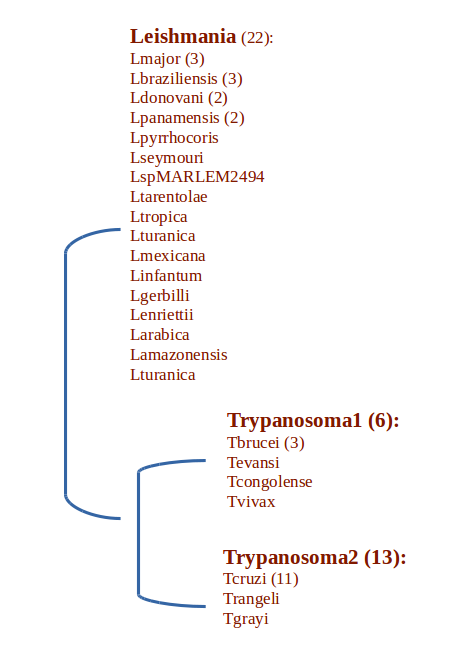
\includegraphics[scale = 0.5]{treeClades.png}}
  \caption[]{TriTryp genomes clustered into three classes of Leishmania(L), Trypanosoma1(T1), and Trypanosoma2(T2). other TriTryp genomes within this tree which does not fit into these categories are labeled as Others(o)}
  \label{fig:tree}
\end{figure}

\subsection{Gene Cluster}
We define clusters as a group of two or more genes found within a genome located within a thousand base pairs of each other. For example, cluster "IVQRLTRKGW" is a sequence of genes shown with their one letter amino acid code which are located on same double stranded sequence of a genome and are within a 1000bp of each other. Also the orientation of a cluster is shown as a sequence of $+$s and $-$s which refer to the strand of each gene within the cluster, in order. for instance the orientation of cluster "IVQRLTRKGW" can be shown as $"+-----++-+"$.

%------------------------------------------------------------------------------------------------------
% Background
%------------------------------------------------------------------------------------------------------


\section{\textbf{1. Predicting and annotating tRNA gene models}}
From Tritrypdb \cite{Aslett2010TriTrypDBAF}, we downloaded the version 41 of 46 TryTryp genomes released on 2018-12-05. The quality of sequenced genomes are compared based on number of sequence fragments relative to their length as shown in figure~\ref{fig:gallery}. Later, We annotated tRNA genes for the sequenced TryTryp genomes using two computational methods for tRNA prediction, tRNAscan-SE (TSE) \cite{trnascan} and Aragorn (ARA) \cite{aragorn}. We integrated the result of both gene finders by keeping the union of tRNA gene predictions generated by tRNAscan-SE v2.0 using defult options (Lowe and Eddy 1997) and Aragorn v1.2.38 using options -i116 -t -br -seq -w -e -l -d (Laslett and Canback 2004). Genes with overlapped coordinate were considered as one gene. However, the identity and exact coordinate of both genefinders were saved seperately to be analysed later. 4381 genes were predicted from which 3597 genes were predicted by both gene finders, 750 genes predicted by ARA only and 34 genes predicted by TSE only. Since Aragorn cannot predict the initiators, we predicted the initiator tRNAs for the genes with anticodon 'CAT' from union of both genefinders Based on Conserved positions of initiators in Eukarya from the study by Christian Marck and Henri Grosjean \cite{tRNomics}.


\begin{figure}[htbp]
  \centering
  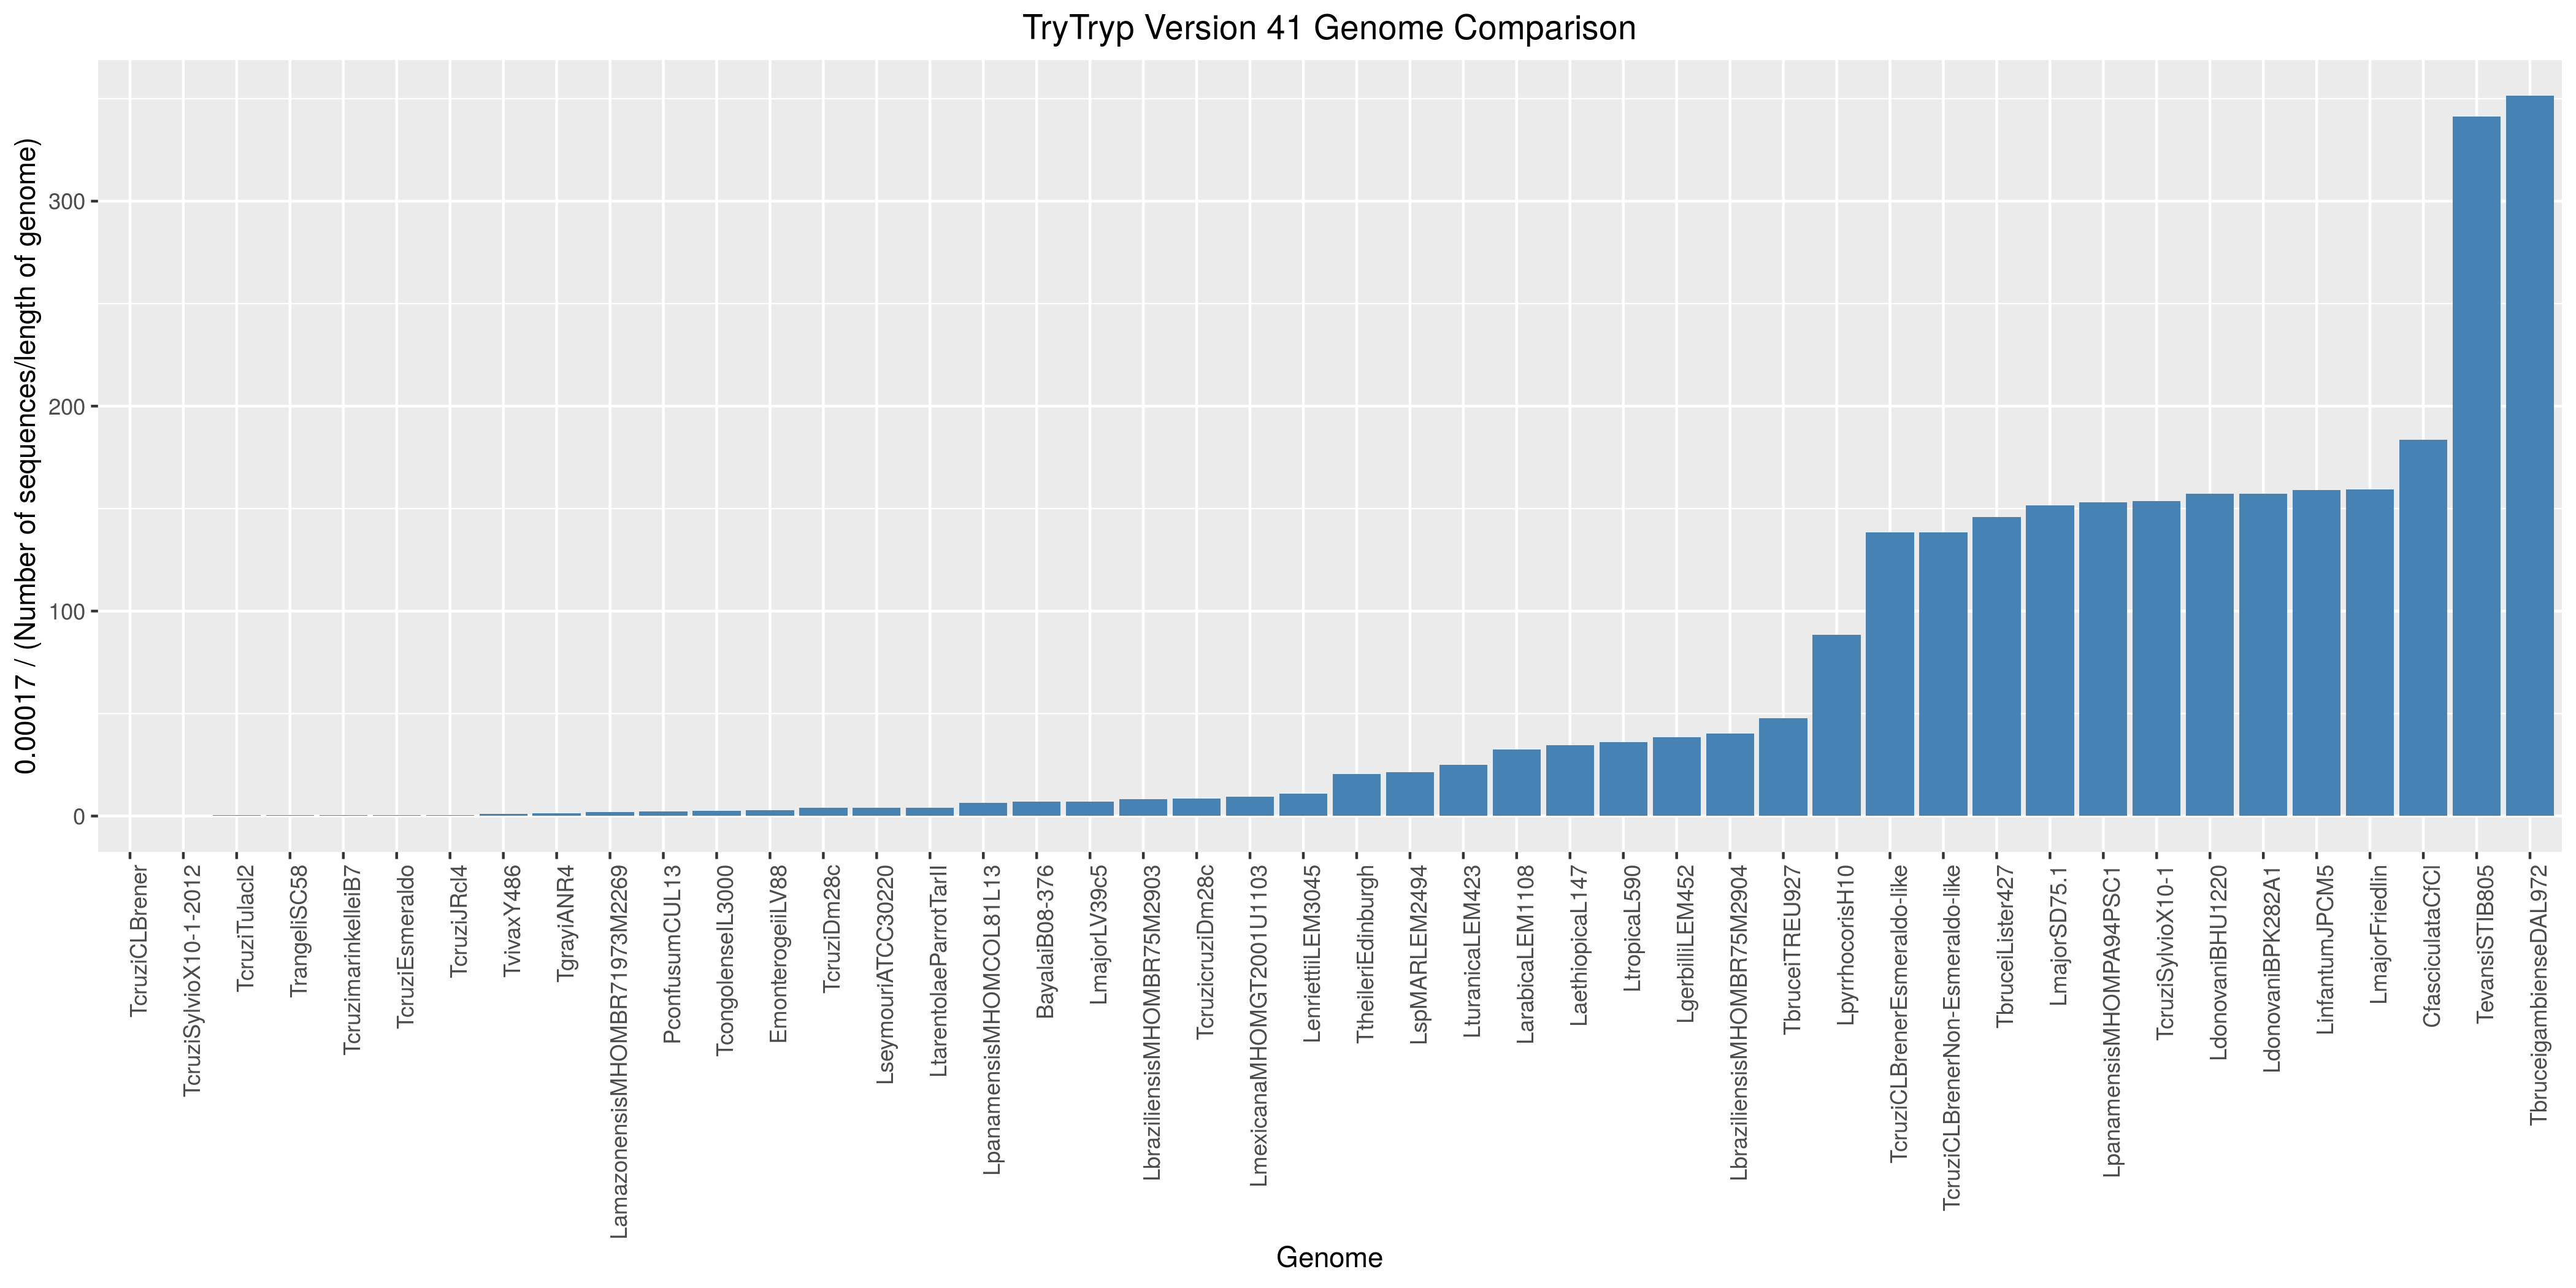
\includegraphics[width=\columnwidth]{GenomeComparisonV41.png}
  \caption[Genome Comparison]{Comparing genomes based on formula ${(\frac{f(x)}{\max(f(x))})}^{-1}$. f(x) = Number of sequences in genome devided by the length of genome. The length of the bars shows quality of genome sequencing.} % The text in the square bracket is the caption for the list of figures while the text in the curly brackets is the figure caption
  \label{fig:gallery}
\end{figure}

%------------------------------------------------------------------------------------------------------
% Initiator tRNA prediction
%------------------------------------------------------------------------------------------------------

\subsection{\textbf{1.2 Initiator tRNA prediction}}
We predicted the initiator tRNAs for the genes with anticodon 'CAT' from union of both tRNAscan (TSE) and Aragorn (ARA) Based on Conserved positions of initiators in Eukarya from the study by CHRISTIAN MARCK and HENRI GROSJEAN. Based on this study we have the fallowing citeria for initiators:
\begin{enumerate}[noitemsep] % [noitemsep] removes whitespace between the items for a compact look
  \item In all eukaryotic tDNA-iMet, positions 11–24 are occupied by C-G, However, eukaryotic elongators
        also prefer C-G at these positions.

  \item Initiator tDNAs from Eukarya use A54 and A60. Some eukaryotic elongators also use either A54 or
        A60 but none (with only one exception) uses both

  \item Initiator tDNA-iMet (CAT) from all domains display the GGG sequence (Mandal et al+, 1996) or,
        very seldom, the AGG sequence at positions 29 to 31, pairing with the complementary CCC or
        CCT sequences at positions 39 to 41

  \item Another domain-specific feature in all eukaryotic initiators is the systematic nonoccupancy of all
        optional positions of the D-loop (17, 17a, 20a, and 20b) whereas in elongators, only position 17a is always unoccupied.

  \item At position 20, A is strictly conserved in all eukaryotic initiators
\end{enumerate}
To investigate all these features first we used CAT genes from the gene set. We had 188 genes with anticodon CAT from which 4 genes were found by only ARA and the rest were found by both genefinders. Later, we aligned all the genes from the intersection of ARA and TSE along with 4 CAT genes found only by ARA. in the result gene set, we had 185 CAT genes left (3 of them which were found by ARA were removed during the alignment due to unusual structure. these genes were also low score ARA genes with ARA score of less than 102). Later we clustered these 185 CAT genes using Levenshtein (edit) distance between gene sequences and Ward.D2 method to measure the dissimilarity between each two clusters. We ended up with three clusters. Table \ref{table:1} investigates each of these features in each column. from this table we see that only tRNA genes in cluster 1 have almost all the conserved features for eukaryotic initiators. So, we marked these genes as initiators represented with letter X in our gene file. The only CAT gene found by ARA was is included in cluster 3. Further, to verify these 76 initiator, we compared them to the CAT genes marked as initiators (iMet) by TSE. There were 76 genes marked as initiator by TSE which matched with all the CAT genes we marked as initiator.


\begin{table}[htbp]
  \caption{Table of CAT clusters to show how many tRNA genes in each cluster satisfy each feature}
  \begin{adjustbox}{width=\textwidth,center}
    %\caption{Table of Grades}
    %\centering
    \begin{tabular}{|l|lllllllll|}
      \hline
      Clusters & \# tRNAs & 11–24(C-G) & 54-60(A-A)(T-T) & 1-72(A-T) & 29-31(GGG) & 39-41(CCC/CCT) & \#  posisInDloop & 20A & distanceRange \\
      \hline
      Cluster1&76&76&76&76&76&76&7&75\\
      Cluster2&95&95&2&0&0&0&8&0\\
      Cluster3&14&2&13&0&0&0&1&0\\
      \hline
    \end{tabular}
    \label{table:1}
  \end{adjustbox}
\end{table}

% Gene summerize table 

% pseudo | truncated genes 
\subsection{\textbf{Detailed Gene Annotation}}
The fallowing is a list of ambiguities in predicted genes by two gene finders which needs to be resolved in order to integrate and filter out the untrusted genes.
\begin{itemize}
  \item[1.] Genes found by Aragorn only
  \item[2.] Genes found by tRNAScan-SE only
  \item[3.] Genes marked as pseudo or truncated by TSE
  \item[4.] Genes with unidentified identity by both gene finders
  \item[5.] Genes with different identities between two gene finders
\end{itemize}


%------------------------------------------------------------------------------------------------------
% Pseudo Genes
%------------------------------------------------------------------------------------------------------

\subsection{\textbf{1.3 Pseudo Genes}}

There are 43 genes marked as pseudo or truncated by TSE. Table \ref{table:pseudo1} shows the number of pseudo and truncated genes from our initial gene set. Among these, 4 genes found only by TSE with score of between 20-30 (genes which barely passed the score threshold (20) by TSE) were not assigned any identity or anticodon. From 39 remain genes, 15 genes were found by both gene finders and the rest (24 genes) were predicted by only TSE. In order to verify these 39 genes with assigned identity, we analyzed them among clusters. Table \ref{table:pseudo2} shows the pseudo/truncated genes within clusters along with singletons. Pseudo genes are marked with lower letter characters. Table \ref{table:pseudo3} shows the sets of clusters which are similar to the  pseudo containing clusters with possible variations including deletion, duplicated, insertion and inversion. From these tables we can see that all the pseudo containing clusters except for cluster "Eye" are similar to other non-pseudo gene containing clusters, which means that these genes have potentially lost some functionalities due to structural variations in chunks of genomes including inversions and duplication. Also, 21 of these pseudo genes appeared as singletons from which 8 genes were found by both gene finders. Also, one of the the pseudo genes found by both gene finders has been assigned with two different anticodon/identity, I (by TSE) and D (by ARA).


\begin{table}[htbp]
  \caption{Genes labeled as pseudo, truncated or both by TSE}
  \begin{adjustbox}{width=7cm,center}
    \begin{tabular}{|c||c||c|}
      \hline
      pseudo & truncated & truncated,pseudo \\
      \hline
      28     & 11        & 4                \\
      \hline
    \end{tabular}
    \label{table:pseudo1}
  \end{adjustbox}
\end{table}

\begin{table}[htbp]
  \caption{Table of pseudo-gene containing clusters along with singleton pseudo genes. Column genes foundby shows which gene finder predicted each gene within the cluster, in order. Column cluster foundby shows whether the whole cluster has been found by both gene finders or TSE only. Cluster i/d refers to genes found by both genefinders with different assigned identity. TSE identity of I and ARA identity of D.}
  \begin{adjustbox}{width=\textwidth,center}
    %\caption{Table of Grades}
    %\centering
    \begin{tabular}{|l|c|l|l|}
      \hline
      cluster    & frequency & genes foundby                                   & cluster foundby \\
      \hline\hline
      DSa        & 1         & both-both-both                                  & both            \\
      Eye        & 1         & both-tse-both                                   & tse             \\
      f          & 4         & both,tse                                        & both,tse        \\
      fIQ        & 1         & tse-both-both                                   & tse             \\
      FIQa       & 1         & both-both-both-tse                              & tse             \\
      FIQFIQafIQ & 1         & both-both-both-both-both-both-tse-tse-both-both & tse             \\
      i          & 1         & both                                            & both            \\
      i/d        & 2         & both                                            & both            \\
      IQl        & 1         & both-both-both                                  & both            \\
      k          & 3         & both                                            & both            \\
      lS         & 1         & both-both                                       & both            \\
      Nk         & 1         & both-tse                                        & tse             \\
      p          & 1         & tse                                             & tse             \\
      PTn        & 1         & both-both-tse                                   & tse             \\
      r          & 1         & both                                            & both            \\
      s          & 7         & tse                                             & tse             \\
      sK         & 1         & both-both                                       & both            \\
      sKHSk      & 1         & both-both-both-both-tse                         & tse             \\
      t          & 1         & tse                                             & tse             \\
      YTyTTy     & 2         & both-both-tse-both-both-tse                     & tse             \\
      z          & 1         & both                                            & both            \\
      \hline
    \end{tabular}
    \label{table:pseudo2}
  \end{adjustbox}
\end{table}


\begin{table}[htbp]
  \caption{Sets of pseudo containing clusters with potential variations between clusters of each set including duplication, deletion, inversion. There are three genome classes T, L and O which refer to Trypanosoma, Leishmania and Other genomes, in order. Clusters with same set number are considered similar. Three last column shows the orientation of genes within clusters for each class of genomes.}
  \begin{adjustbox}{width=\textwidth,center}
    \begin{tabular}{|c||c|} \hline
      %%%%%% Title row starts here
      \begin{tabular}{l ccccc}
        %\hline
        clusters  & set & Genomeclass & Tdirs           & Ldirs  & Odirs  \\
        \rowcolor{shadecolor}
        Eye       & 0   & T           & ++-             &        &        \\
        Nk        & 1   & T           & --              &        &        \\
        \rowcolor{white}
        KN        & 1   & L           &                 & +-     &        \\
        ENKRRA    & 1   & O           &                 &        & --++-+ \\
        \rowcolor{shadecolor}
        DSa       & 2   & T           & -++             &        &        \\
        \rowcolor{white}
        ASD       & 2   & LT          & --+             & --+    &        \\
        AS        & 2   & O           &                 &        & +-     \\
        DSA       & 2   & OLT         & -++             & -++    & -++    \\
        ASDD      & 2   & T           & --++            &        &        \\
        DS        & 2   & T           & -+              &        &        \\
        DSV       & 2   & T           & -++             &        &        \\
        \rowcolor{shadecolor}
        YTyTTy    & 3   & L           &                 & ----++ &        \\
        \rowcolor{white}
        YTTY      & 3   & L           &                 & --++   &        \\
        YTY       & 3   & L           &                 & --+    &        \\
        YT        & 3   & LT          & +-              & --     &        \\
        YTRD      & 3   & OL          &                 & ----   & ----   \\
        TY        & 3   & OLT         & +-              & ++     & ++     \\
        \rowcolor{shadecolor}
        lS        & 4   & T           & --              &        &        \\
        \rowcolor{white}
        MEYSL     & 4   & O           &                 &        & ----+  \\
        LS        & 4   & OLT         & --              & --     & --     \\
        SL        & 4   & OLT         & --|++           & ++     & ++     \\
        LSM       & 4   & T           & -+-             &        &        \\
        LSMEMSMYV & 4   & T           & -+-++-+-+       &        &        \\
        LSMEMYV   & 4   & T           & -+-++-+|-+--+-+ &        &        \\
        MEMSL     & 4   & T           & --+-+|-++-+     &        &        \\
        VYMEMSL   & 4   & T           & -+-++-+|-+--+-+ &        &        \\
        %\hline
      \end{tabular} &

      \begin{tabular}{l ccccc}
        %\hline
        clusters   & set & Genomeclass & Tdirs      & Ldirs & Odirs   \\
        \rowcolor{shadecolor}
        FIQa       & 5   & T           & ---+       &       &         \\
        fIQ        & 5   & T           & ---        &       &         \\
        FIQFIQafIQ & 5   & T           & ------+--- &       &         \\
        \rowcolor{white}
        QFIQ       & 5   & T           & ----       &       &         \\
        \rowcolor{shadecolor}
        IQl        & 6   & T           & -++        &       &         \\
        \rowcolor{white}
        ILQ        & 6   & T           & +--        &       &         \\
        ILQI       & 6   & T           & +-++       &       &         \\
        ILQQI      & 6   & T           & +--++      &       &         \\
        IQ         & 6   & T           & -+         &       &         \\
        IQL        & 6   & T           & -++        &       &         \\
        IQQL       & 6   & T           & --++       &       &         \\
        IQQLI      & 6   & T           & --++-      &       &         \\
        QLI        & 6   & LT          & -+-        & +-+   &         \\
        QLIIIII    & 6   & O           &            &       & +-++--+ \\
        \rowcolor{shadecolor}
        PTn        & 7   & T           & -++        &       &         \\
        \rowcolor{white}
        NPTYN      & 7   & L           &            & --+++ &         \\
        YTN        & 7   & O           &            &       & ---     \\
        NYTPN      & 7   & OL          &            & ---++ & ---++   \\
        TN         & 7   & OT          & ++         &       & ++      \\
        NT         & 7   & T           & --         &       &         \\
        NTP        & 7   & T           & --+        &       &         \\
        NY         & 7   & T           & -+         &       &         \\
        PTN        & 7   & T           & -++        &       &         \\
        PTYN       & 7   & T           & -+-+       &       &         \\
        \rowcolor{shadecolor}
        sK         & 8   & T           & --         &       &         \\
        sKHSk      & 8   & T           & -----      &       &         \\
        %\hline
      \end{tabular} \\ \hline
    \end{tabular}
    \label{table:pseudo3}
  \end{adjustbox}
\end{table}


%------------------------------------------------------------------------------------------------------
% Other Unidentified Genes
%------------------------------------------------------------------------------------------------------

\subsection{\textbf{1.4 Other Unidentified Genes}}

There were \textbf{15 genes} from our initial gene set with unassigned identity both genefinders, 9 found by TSE (with score < 30), 4 found by ARA (with scores between 100-101) and 2 found by both (with ARA score of 116,112 and TSE score of 54,51). Three of the 9 genes found by TSE are marked as pseudo and one as truncated. TSE has not been able to assign any anticodon to these genes. However ARA assigned anticodon of length 2 or 4 to these genes. These genes seems to have unusual arm length including unpaired base and/or insertion in their arms.\textbf{ (These 15 genes are excluded in annotation of genes in the fallowing sections which leaves the total number of 4366 genes: 3595 found by both TSE and ARA, 30 genes by TSE only and 741 genes by ARA only)}\\
\emph{(note! we can find the identity of these two genes using the profiles! and look at them within clusters for potential shifts or inversions).}\\

Also, there were 4 genes with identities A,K,Z,E. 1 found by only TSE and 3 found by both genefinders which has 1- 3 letters of N. with TSE score of 60-11 and ARA score of 107-117.

%------------------------------------------------------------------------------------------------------
% Genes found by only one gene finder
%------------------------------------------------------------------------------------------------------


\subsection{\textbf{1.5 Genes found by only one gene finder}}
\subsubsection{1.5.1 ARA only genes}
\textbf{741 genes} of our total initial gene set were found by only ARA. Table \ref{table:ara1} shows the ARA-only genes within clusters along with ARA-only  singletons. ARA -only genes are shown written in lower case letters. Among these genes 20 are within clusters and the rest appeared as singletons. Column \#similar shows number of times each of these ARA-only-gene containing cluster sequences has appeared as subsequence of other clusters made from non-ara-only genes. Last column shows the number of each ara-only gene within the clusters (or singletons) with score of > 106. Based on these two columns, we can see that ara-only-genes which are complementing already seen clusters (clusters that have occurred many times shown in column similar), have higher scores than most of the ara-only singletons genes. However, the ara-only gene containing clusters which have not been seen in other clusters (their \#similar is 0 or 1), have relatively low scores (lower than 107). This shows that using a cutoff score of 107 for ARA genes will keep 36 genes which are potentially most of the reliable ara-only genes figure \ref{fig:aratsescore}a. Table \ref{table:ara2} shows few sample of these similar clusters.
\emph{(note: the sequences of these 20 genes are potentially same as already found genes by TSE and ARA, which were missed by TSE. this should be checked!)  }



\begin{table}[htbp]
  \caption{Table of ara-only-gene containing clusters and singletons. column \#similar shows number of times cluster sequence has appeared as subsequence of other clusters made from the non-ara-only genes from our initial gene set. Last column shows the number of occurances of the ara-only gene within the clusters (or singletons) with score of > 106. this column will be used later for assigning a cutoff score for ara genes. $\star$ in the last columns shows an except. Cluster sl has been found as substring of 22 clusters, however its genes have scores lower than 107. the score for these two genes are 106,105 in order which is close to the threshold.}
  \begin{adjustbox}{center}
    %\caption{Table of Grades}
    %\centering
    \begin{tabular}{|l|c|c|c|}
      \hline
      cluster & frequency & \# similar & \# genes with score > 106 \\
      \hline\hline
      dSA     & 1         & 37         & 1                         \\
      fRA     & 1         & 4          & 1                         \\
      rh      & 1         & 25         & 1                         \\
      gT      & 1         & 29         & 1                         \\
      lA      & 2         & 24         & 2                         \\
      lI      & 1         & 26         & 1                         \\
      sl      & 1         & 22         & $\star$                   \\%(score were 105 and 106)\\
      tt      & 1         & 14         & 1                         \\
      \rowcolor{shadecolor}
      aE      & 1         & 1          & 0                         \\
      \rowcolor{lightgray}
      pppp    & 1         & 0          & 0                         \\
      \rowcolor{lightgray}
      Ek      & 1         & 0          & 0                         \\
      \rowcolor{lightgray}
      Za      & 1         & 0          & 0                         \\
      \rowcolor{lightgray}
      Zr      & 1         & 0          & 0                         \\
      $\#$    & 2         & -          & 0                         \\
      a       & 43        & -          & 2                         \\
      c       & 22        & -          & 1                         \\
      d       & 13        & -          & 0                         \\
      e       & 31        & -          & 1                         \\
      f       & 19        & -          & 1                         \\
      g       & 109       & -          & 2                         \\
      h       & 48        & -          & 3                         \\
      i       & 41        & -          & 1                         \\
      k       & 6         & -          & 1                         \\
      l       & 38        & -          & 3                         \\
      m       & 4         & -          & 0                         \\
      n       & 17        & -          & 0                         \\
      o       & 2         & -          & 0                         \\
      p       & 24        & -          & 0                         \\
      q       & 13        & -          & 0                         \\
      r       & 69        & -          & 1                         \\
      s       & 130       & -          & 7                         \\
      t       & 28        & -          & 2                         \\
      v       & 41        & -          & 0                         \\
      w       & 5         & -          & 1                         \\
      y       & 12        & -          & 0                         \\
      z       & 4         & -          & 0                         \\

      \hline
    \end{tabular}
    \label{table:ara1}
  \end{adjustbox}
\end{table}


\begin{table}[htbp]
  \caption{Sets of ara-only-gene containing clusters with potential variations between clusters of each set including duplication, deletion, inversion. There are three genome classes T, L and O which refer to Trypanosoma, Leishmania and Other genomes, in order. Clusters with same set number are considered similar. Three last column shows the orientation of genes within clusters for each class of genomes.}
  \begin{adjustbox}{width=\textwidth,center}
    \begin{tabular}{|c||c|} \hline
      %%%%%% Title row starts here
      \begin{tabular}{l ccccc}
        %\hline
        clusters     & set & Genomeclass & Tdirs  & Ldirs     & Odirs \\
        \rowcolor{shadecolor}
        RRAE         & 1   & O           &        &           & --++  \\
        EARR         & 1   & L           &        & --++      &       \\
        \textbf{Ek}  & 1   & L           &        & --        &       \\
        \rowcolor{white}
        dSA          & 4   & T           & -++    &           &       \\
        DSA          & 4   & OLT         & -++    & -++       & -++   \\
        DSV          & 4   & T           & -++    &           &       \\
        ASD          & 4   & LT          & --+    & --+       &       \\
        ASDD         & 4   & T           & --++   &           &       \\
        DS           & 4   & T           & -+     &           &       \\
        \rowcolor{shadecolor}
        \textbf{fRA} & 1   & T           & -++    &           &       \\
        FRA          & 1   & T           & -++    &           &       \\
        ARF          & 1   & T           & --+    &           &       \\
        ARFARF       & 1   & T           & --+--+ &           &       \\
        \rowcolor{white}
        \textbf{gT}  & 2   & T           & -+     &           &       \\
        GT           & 2   & OLT         & -+     & ++        & ++    \\
        GTGP         & 2   & L           &        & +--+|++-+ &       \\
        GTGPVK       & 2   & L           &        & +--+++    &       \\
        GTP          & 2   & L           &        & +-+       &       \\
        PGTTG        & 2   & L           &        & -++--     &       \\
        TG           & 2   & OT          & -+     &           & --    \\
        TGP          & 2   & OL          &        & --+       & --+   \\
        PTG          & 2   & L           &        & ---       &       \\
        %\hline
      \end{tabular} &

      \begin{tabular}{l ccccc}
        %\hline
        clusters    & set & Genomeclass & Tdirs           & Ldirs & Odirs  \\
        \rowcolor{shadecolor}
        pppp        & 2   & T           & ----            &       &        \\
        PP          & 2   & O           &                 &       & -+     \\
        \rowcolor{white}
        \textbf{rh} & 7   & T           & --              &       &        \\
        EVRH        & 7   & OL          &                 & --++  & --++   \\
        FHVRH       & 7   & L           &                 & +--++ &        \\
        RHLP        & 7   & T           & ++++            &       &        \\
        HRVE        & 7   & L           &                 & --++  &        \\
        \rowcolor{shadecolor}
        \textbf{sl} & 5   & T           & --              &       &        \\
        SL          & 5   & OLT         & ++              & ++    & ++     \\
        SLS         & 5   & T           & +--|++-         &       &        \\
        SLMIV       & 2   & L           &                 & -+--+ &        \\
        MEMSL       & 5   & T           & --+-+|-++-+     &       &        \\
        MEYSL       & 5   & O           &                 &       & ----+  \\
        VYMEMSL     & 5   & T           & -+-++-+|-+--+-+ &       &        \\
        LS          & 5   & OLT         & --              & --    & --     \\
        LSM         & 5   & T           & -+-             &       &        \\
        LSMEMSMYV   & 5   & T           & -+-++-+-+       &       &        \\
        LSMEMYV     & 5   & T           & -+-++-+|-+--+-+ &       &        \\
        LSSS        & 5   & O           &                 &       & ----   \\
        LSMIVY      & 2   & O           &                 &       & -+---+ \\
        \rowcolor{white}
        \textbf{Za} & 13  & L           &                 & --    &        \\
        \rowcolor{shadecolor}
        \textbf{Zr} & 1   & O           &                 &       & --     \\
        %\hline
      \end{tabular} \\ \hline
    \end{tabular}
    \label{table:ara2}
  \end{adjustbox}
\end{table}


\subsubsection{1.5.2 TSE only genes}
TSE predicted \textbf{30 genes} which were not predicted by ARA. 29 of these genes are very low scored TSE genes scored from 20 to 48. and one gene with score 58. Table \ref{table:tse1} shows the frequency of these genes as three sets of pseudo, truncated, and truncated,pseudo. the last three sets has already been annotated. Table \ref{table:tse2} shows a summary of TSE-only genes as clusters. Genes appeared as singletons have very low score, however genes appered within the clusters have relatively higher scores. cluster VYIMLs which contains gene S found by only TSE has been seen before as exact same clusters with genes found by both genefinders. Also, cluster QLIiIII which contains gene i, has also appeared many times as form of QLI, ILQ and other similar clusters which can be validify the existence of this TSE-only gene. Figure \ref{fig:aratsescore}b shows the TSE scores of genes found by TSE.


\begin{table}[htbp]
  \caption{TSE-only genes}
  \begin{adjustbox}{width=7cm,center}
    %\caption{Table of Grades}
    %\centering
    \begin{tabular}{|cccc|}
      \hline
      others & pseudo & truncated & truncated,pseudo \\
      \hline
      6      & 17     & 5         & 2                \\
      \hline
      28-58  & 20-38  & 28-47     & 22-25            \\
      \hline
    \end{tabular}
    \label{table:tse1}
  \end{adjustbox}
\end{table}


\begin{table}[htbp]
  \caption{TSE-only genes}
  \begin{adjustbox}{width=5cm,center}
    %\caption{Table of Grades}
    %\centering
    \begin{tabular}{|ccc|}
      \hline
      cluster & frequency & TSE score \\
      \hline\hline
      g       & 2         & 28        \\
      i       & 1         & 33        \\
      k       & 1         & 24        \\
      QLIiIII & 1         & 58        \\
      VYIMLs  & 1         & 47        \\
      \hline
    \end{tabular}
    \label{table:tse2}
  \end{adjustbox}
\end{table}

\begin{figure}[H]%
  \centering
  \subfloat[]{{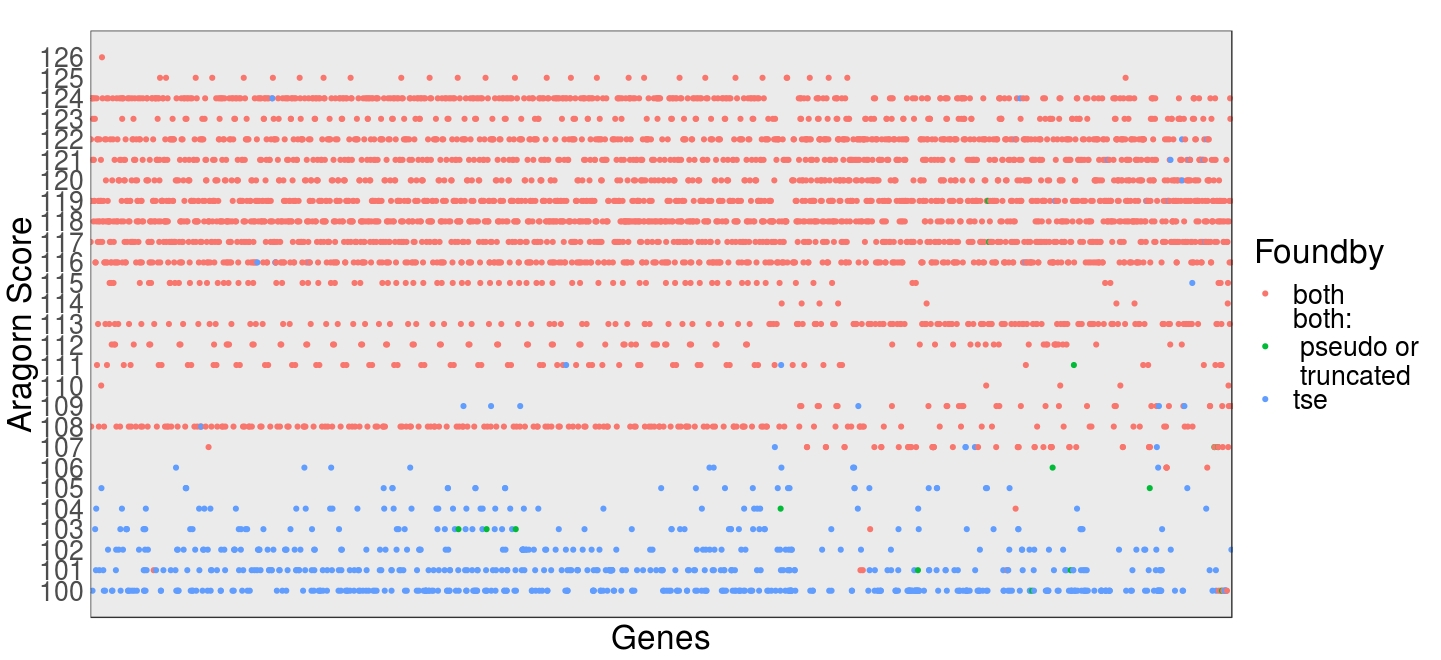
\includegraphics[width=8cm]{araScores.jpeg}}}%
  %\qquad
  \subfloat[]{{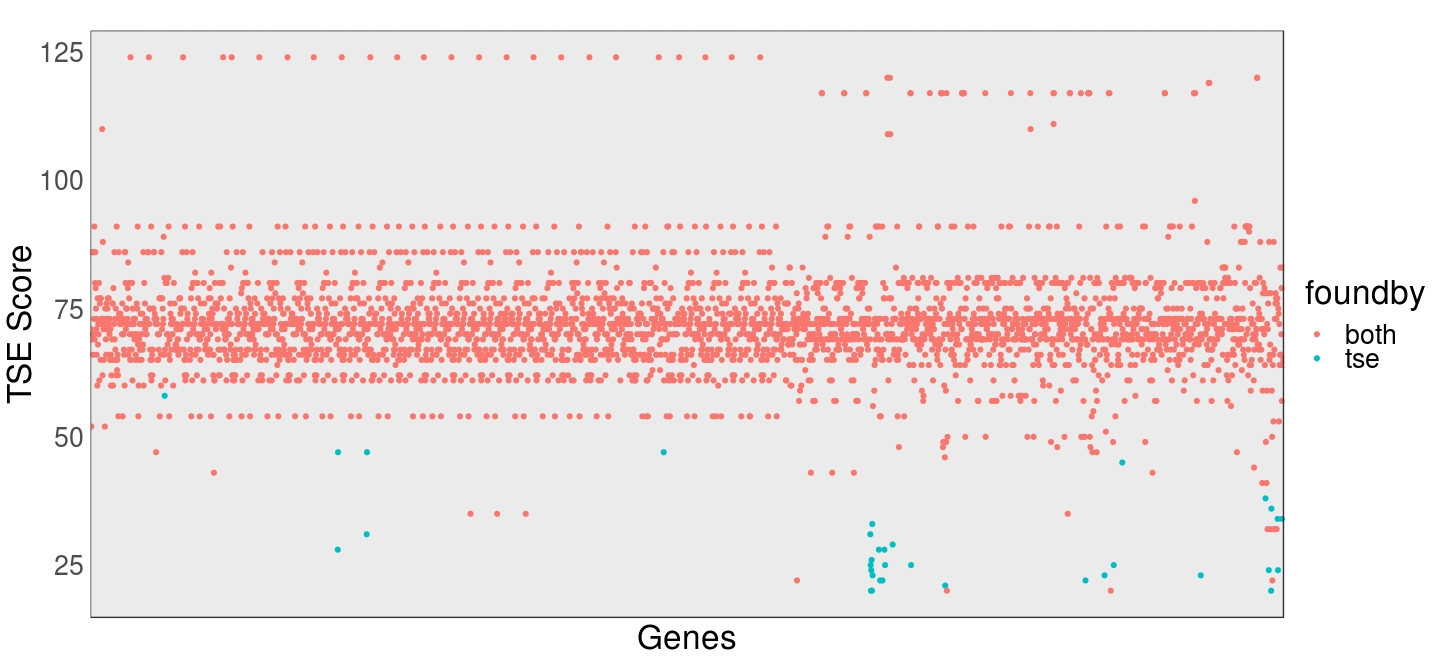
\includegraphics[width=8cm]{tseScores.jpeg}}}%
  \caption{a) ARA score of genes found by both genefinders TSE and ARA, and genes found by only ARA. b) TSE score of genes found by both genefinders and genes found by only TSE}%
  \label{fig:aratsescore}%
\end{figure}


%------------------------------------------------------------------------------------------------------
% Deviations between two gene finders
%------------------------------------------------------------------------------------------------------


\newpage
\subsection{\textbf{1.6 Deviations between two gene finders}}
%------------------------------------------------------------------------------------------------------
% Deviations between two gene finders
%------------------------------------------------------------------------------------------------------
Deviation between two gene finders for the predicted genes is defined in form of fallowing question:
Assuming two genes: A1 (predicted by TSE with identity I1) and B (predicted by ARA with identity I2) which I1 can be equal to I2 or not. The coordinates of A and B overlaps, However, there is a small displacement at the 3' and/or 5' ends of these genes. We say that these two genes are one gene (lets call it gene A) with different predicted structure by two gene finders which had caused the displacement and potentially the identity disagreement. The question is which coordinate and which identity best describe gene A? We will approach this problem in two cases described in next two sections for TriTryp genes:
\begin{itemize}
  \item[a.] Genes with unmatched Identity
  \item[b.] End displacement between two genefinders
\end{itemize}
\subsubsection{\textbf{1.6.1 Genes with unmatched Identity}}
From \textbf{3595 genes} found by both gene finders there are 35 genes with mismatched identity by TSE and ARA. Table \ref{table:undet2} shows the frequency of clusters which contains each of these ambiguities. From this table we see that for clusters of length > 2, which contain an ambiguity, have been always appeared with this ambiguity across different genomes.

\begin{table}[hbt]
  \caption{35 genes with unmatch identity/anticodon reported by ARA and TSE. first row shows the ambiguities with the format <ara identity| tse identity>}
  \begin{adjustbox}{scale=0.9,center}
    \begin{tabular}{|c|cccccccc|}
      \hline
      \rowcolor{shadecolor}
      Ambiguity & (D|I) & (L|?) & (L|E) & (L|M) & (N|Y) & (O|M) & (S|R) & (W|G) \\
      \hline
      Frequency & 5     & 3     & 1     & 9     & 11    & 2     & 1     & 3     \\
      \hline
    \end{tabular}
    \label{table:undet1}
  \end{adjustbox}
\end{table}


\begin{table}[htbp]
  \caption{Table of clusters and singletons which contain the Undetermined-indentity genes. column \#similar shows number of times cluster sequence has appeared as subsequence of other clusters made from the non-ara-only genes from our initial gene set.}
  \begin{adjustbox}{width=\textwidth,center}
    %\caption{Table of Grades}
    %\centering
    \begin{tabular}{|lcclccccc|}
      \hline

      TSE Cluster & TSE Cluster Freq & Ambiguity & ARA Cluster & ARA Cluster Freq & arascore & tsescore     & \#ARAsimilar & \#TSEsimilar \\
      \hline\hline
      e           & 1                & (L|E)     & l           & 1                & 113      & 48           & 327          & 150          \\
      gV          & 2                & (W|G)     & wV          & 2                & 113      & 54,66        & 0            & 0            \\
      i           & 5                & (D|I)     & d           & 5                & 115,101  & 49,20$\star$ & 103          & 161          \\
      LSMEMSMyV   & 1                & (N|Y)     & LSMEMSMnV   & 1                & 108      & 72           & 0            & 0            \\
      LSMEMyV     & 5                & (N|Y)     & LSMEMnV     & 5                & 108      & 72           & 0            & 0            \\
      m           & 2                & (O|M)     & o           & 2                & 112      & 47           & 0            & 74           \\
      m           & 9                & (L|M)     & l           & 9                & 112      & 50           & 327          & 74           \\
      rV          & 1                & (S|R)     & sV          & 1                & 113      & 43           & 7            & 3            \\
      ?V          & 3                & (L|?)     & lV          & 3                & 113      & 43           & 1            & 215          \\
      Vg          & 1                & (W|G)     & Vw          & 1                & 113      & 54           & 0            & 2            \\
      Vy          & 1                & (N|Y)     & Vn          & 1                & 101      & 60           & 0            & 6            \\
      VyMEMSL     & 3                & (N|Y)     & VnMEMSL     & 3                & 108      & 72           & 0            & 0            \\
      yV          & 1                & (N|Y)     & nV          & 1                & 108      & 72           & 0            & 1            \\

      \hline
    \end{tabular}
    \label{table:undet2}
  \end{adjustbox}
\end{table}

continues...\\

%------------------------------------------------------------------------------------------------------
% Deviations between two gene finders
%------------------------------------------------------------------------------------------------------

\subsubsection{1.6.2 End displacement between two genefinders}
continues...\\
%------------------------------------------------------------------------------------------------------
% Deviations between two gene finders
%------------------------------------------------------------------------------------------------------

\section{2 Summery of Final Gene Set Annotation}
We made the final gene set data by removing genes with TSE score of less than 50 and genes with ARA score of less than 107. The cutoff score is set based on the ARA and TSE score distribution shown in figure \ref{fig:aratsescore}. This cutoff score as shown in section 1.5 will keep the most trusted genes found by only one of the gene finders (Genes appeared within common clusters across genomes which also complement their clusters to look like other clusters). It will only remove 43 of our genes from intersection set from which 13 are pseudo and/or truncated genes, 10 genes have different identities by two genefinders and 20 other genes removed are shown in table\ref{table:removedgenes}. in the remained gene set, there were 30 genes including: pseudo|truncated genes, genes with unmatched identity, genes with unassigned identity|anticodon by any of genefinders, and genes with letter N in their sequence(we had 4 of these genes). 20 of these genes are marked as genes with vague identity (shown as ??), and the other 10 genes are kept with their TSE identity. These 10 genes were identified as Y by TSE and N by ARA (Genes with ambiguty (y|n)). These genes were manually compare to the other identified genes with identity n and y found by both gene finders. In all cases these 10 genes were considerably more similar to the genes marked with identity Y than genes identified as N. Also, by looking at genes as clusters (a group of two or more genes found within a genome located within a thousand base pairs of each other) they were observed in clusters "LSMEM(y|n)V","V(y|n)MEMSL","LSMEMSM(y|n)V", and (y|n)V. Further we observed that there was no occurrence of genes NY or YN within any cluster, however there were 6 occurrences of YV or VY (one of them in cluster EMYV). Hence, we kept these genes as genes of idenity Y. 9 of these genes were idenitfied for organisms of clade T.cruzi which completed the 21 class of predicted tRNA genes for 8 T.cruzi genomes figure \ref{fig:genPerc}. Summary of these 3591 left genes are shown in table \ref{table:genesummery} as three sets. Also, Cluster size distribution of these genes for three categories of TryTryp genomes is visualized as figure \ref{fig:clussize}.

\begin{figure}[H]%
  \centering
  \subfloat[]{{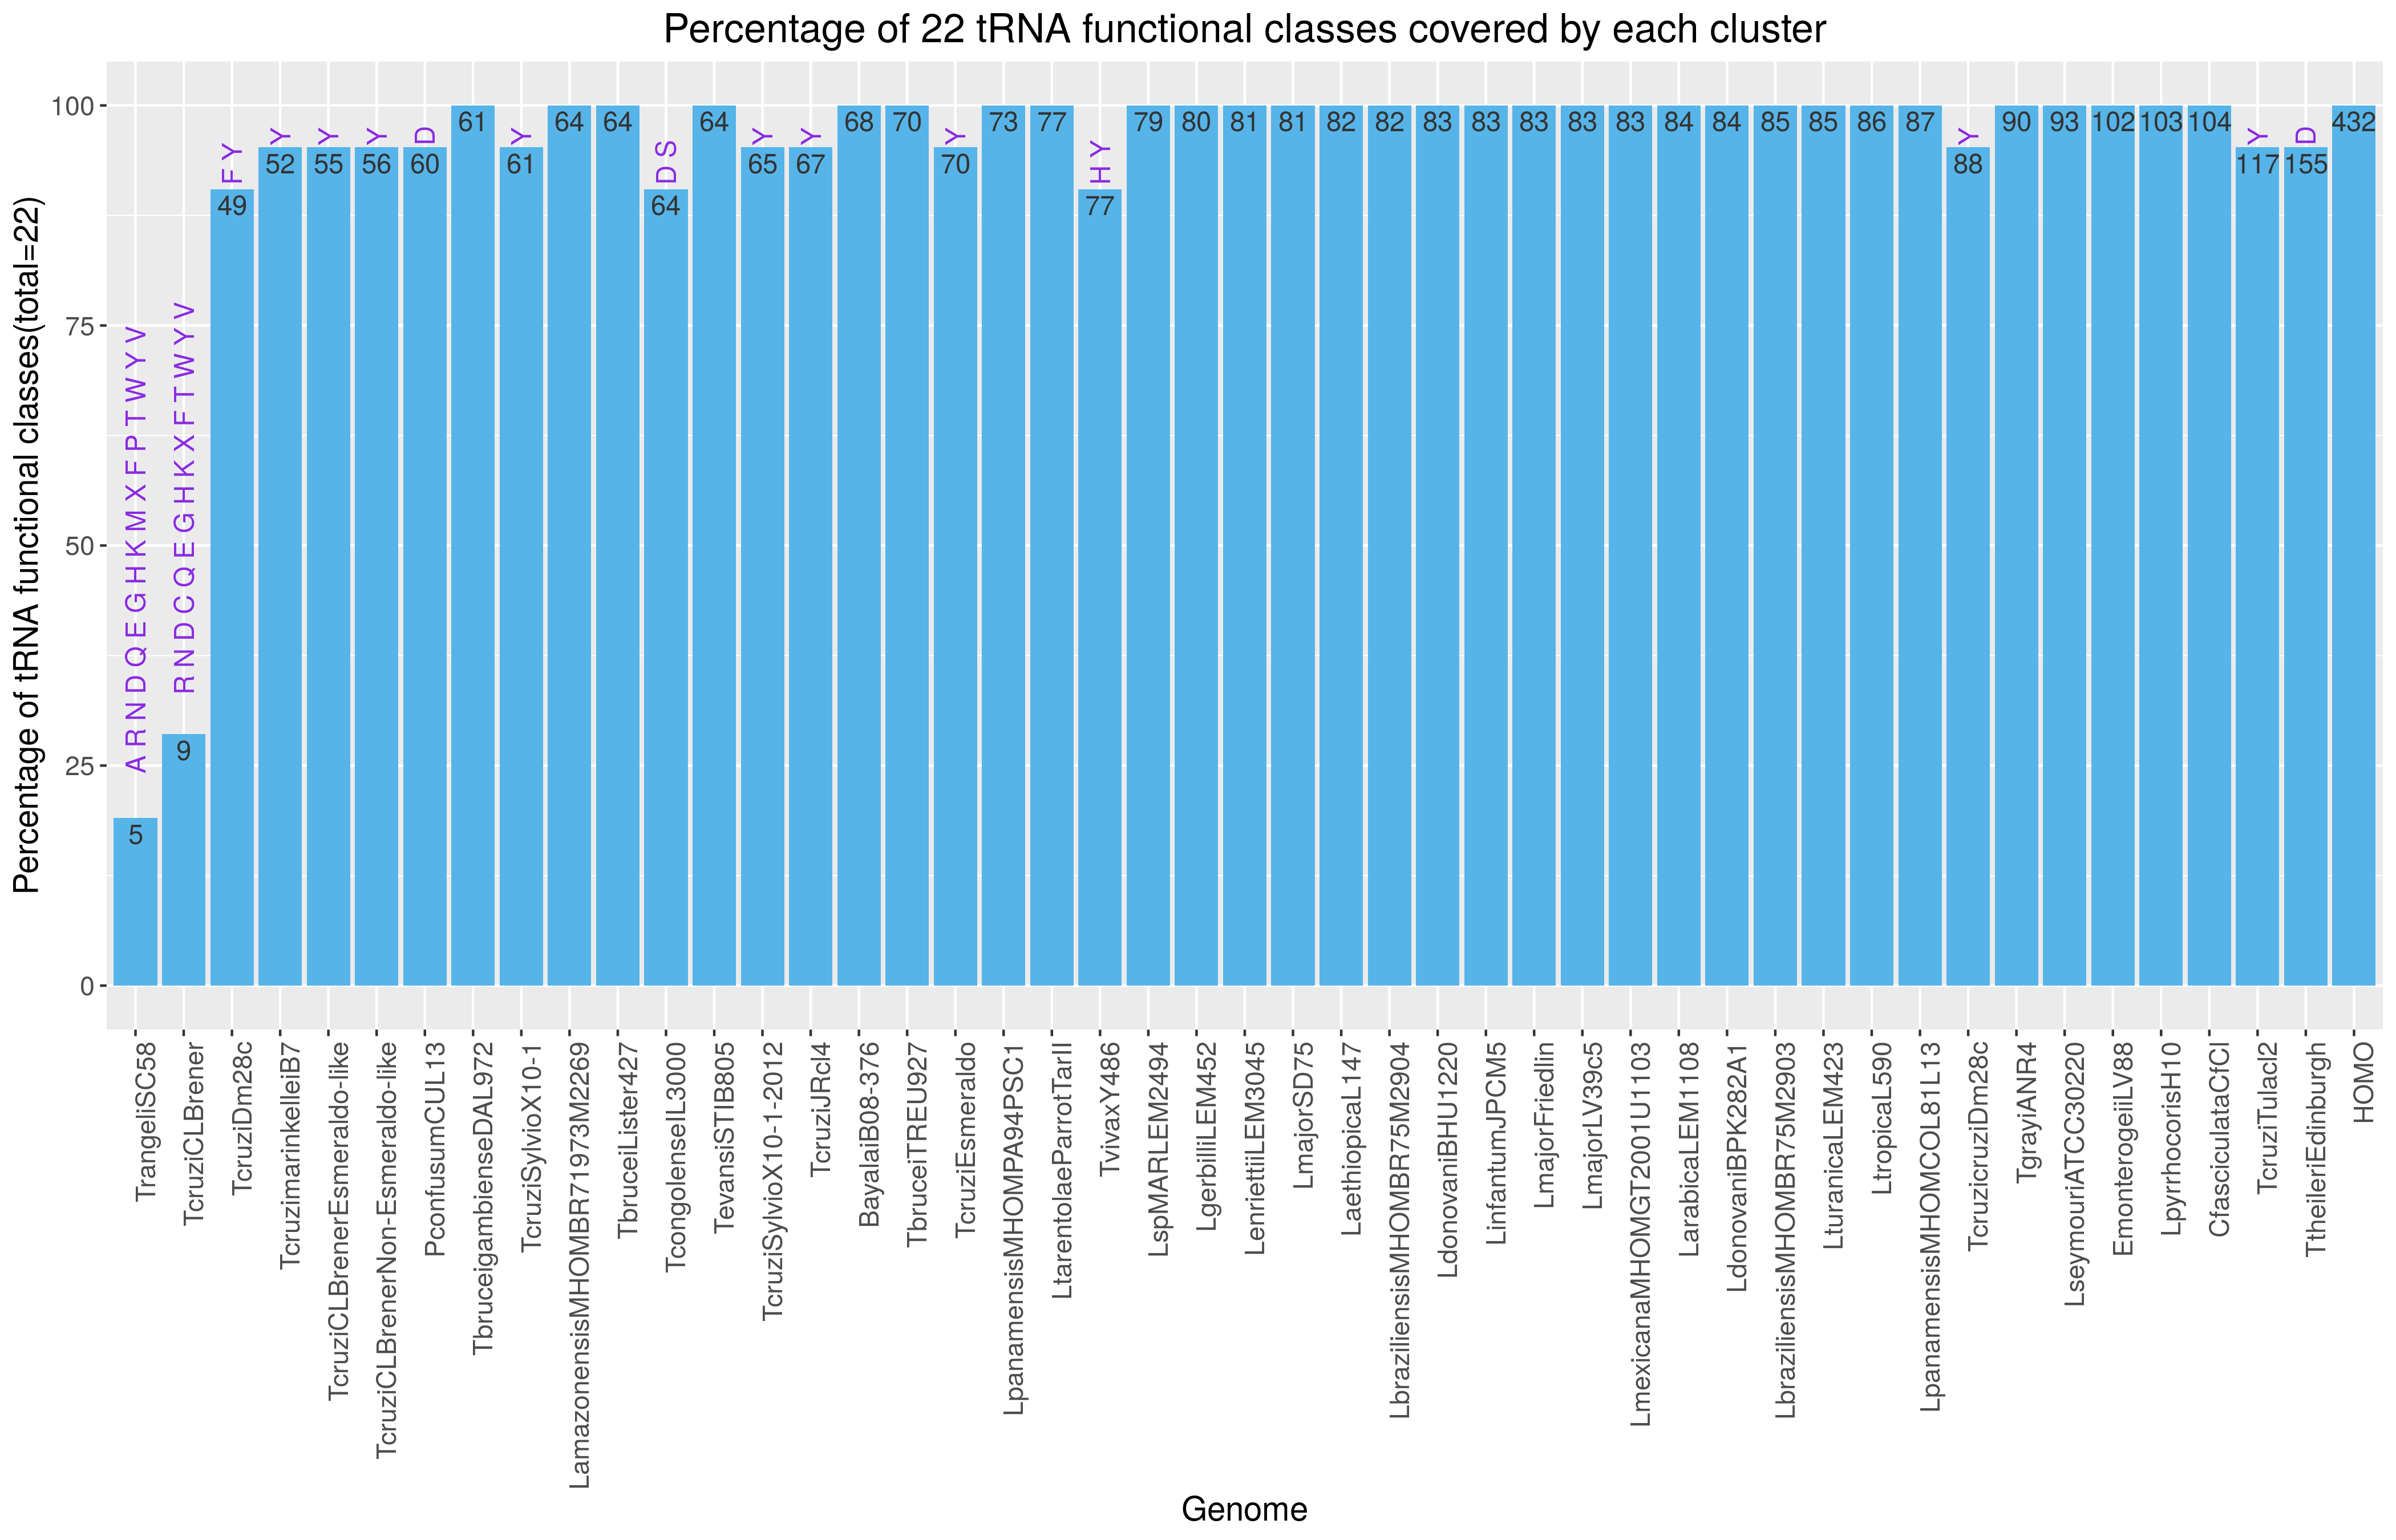
\includegraphics[width=\textwidth]{funcPerc_before.png}}}%
  \\
  \subfloat[]{{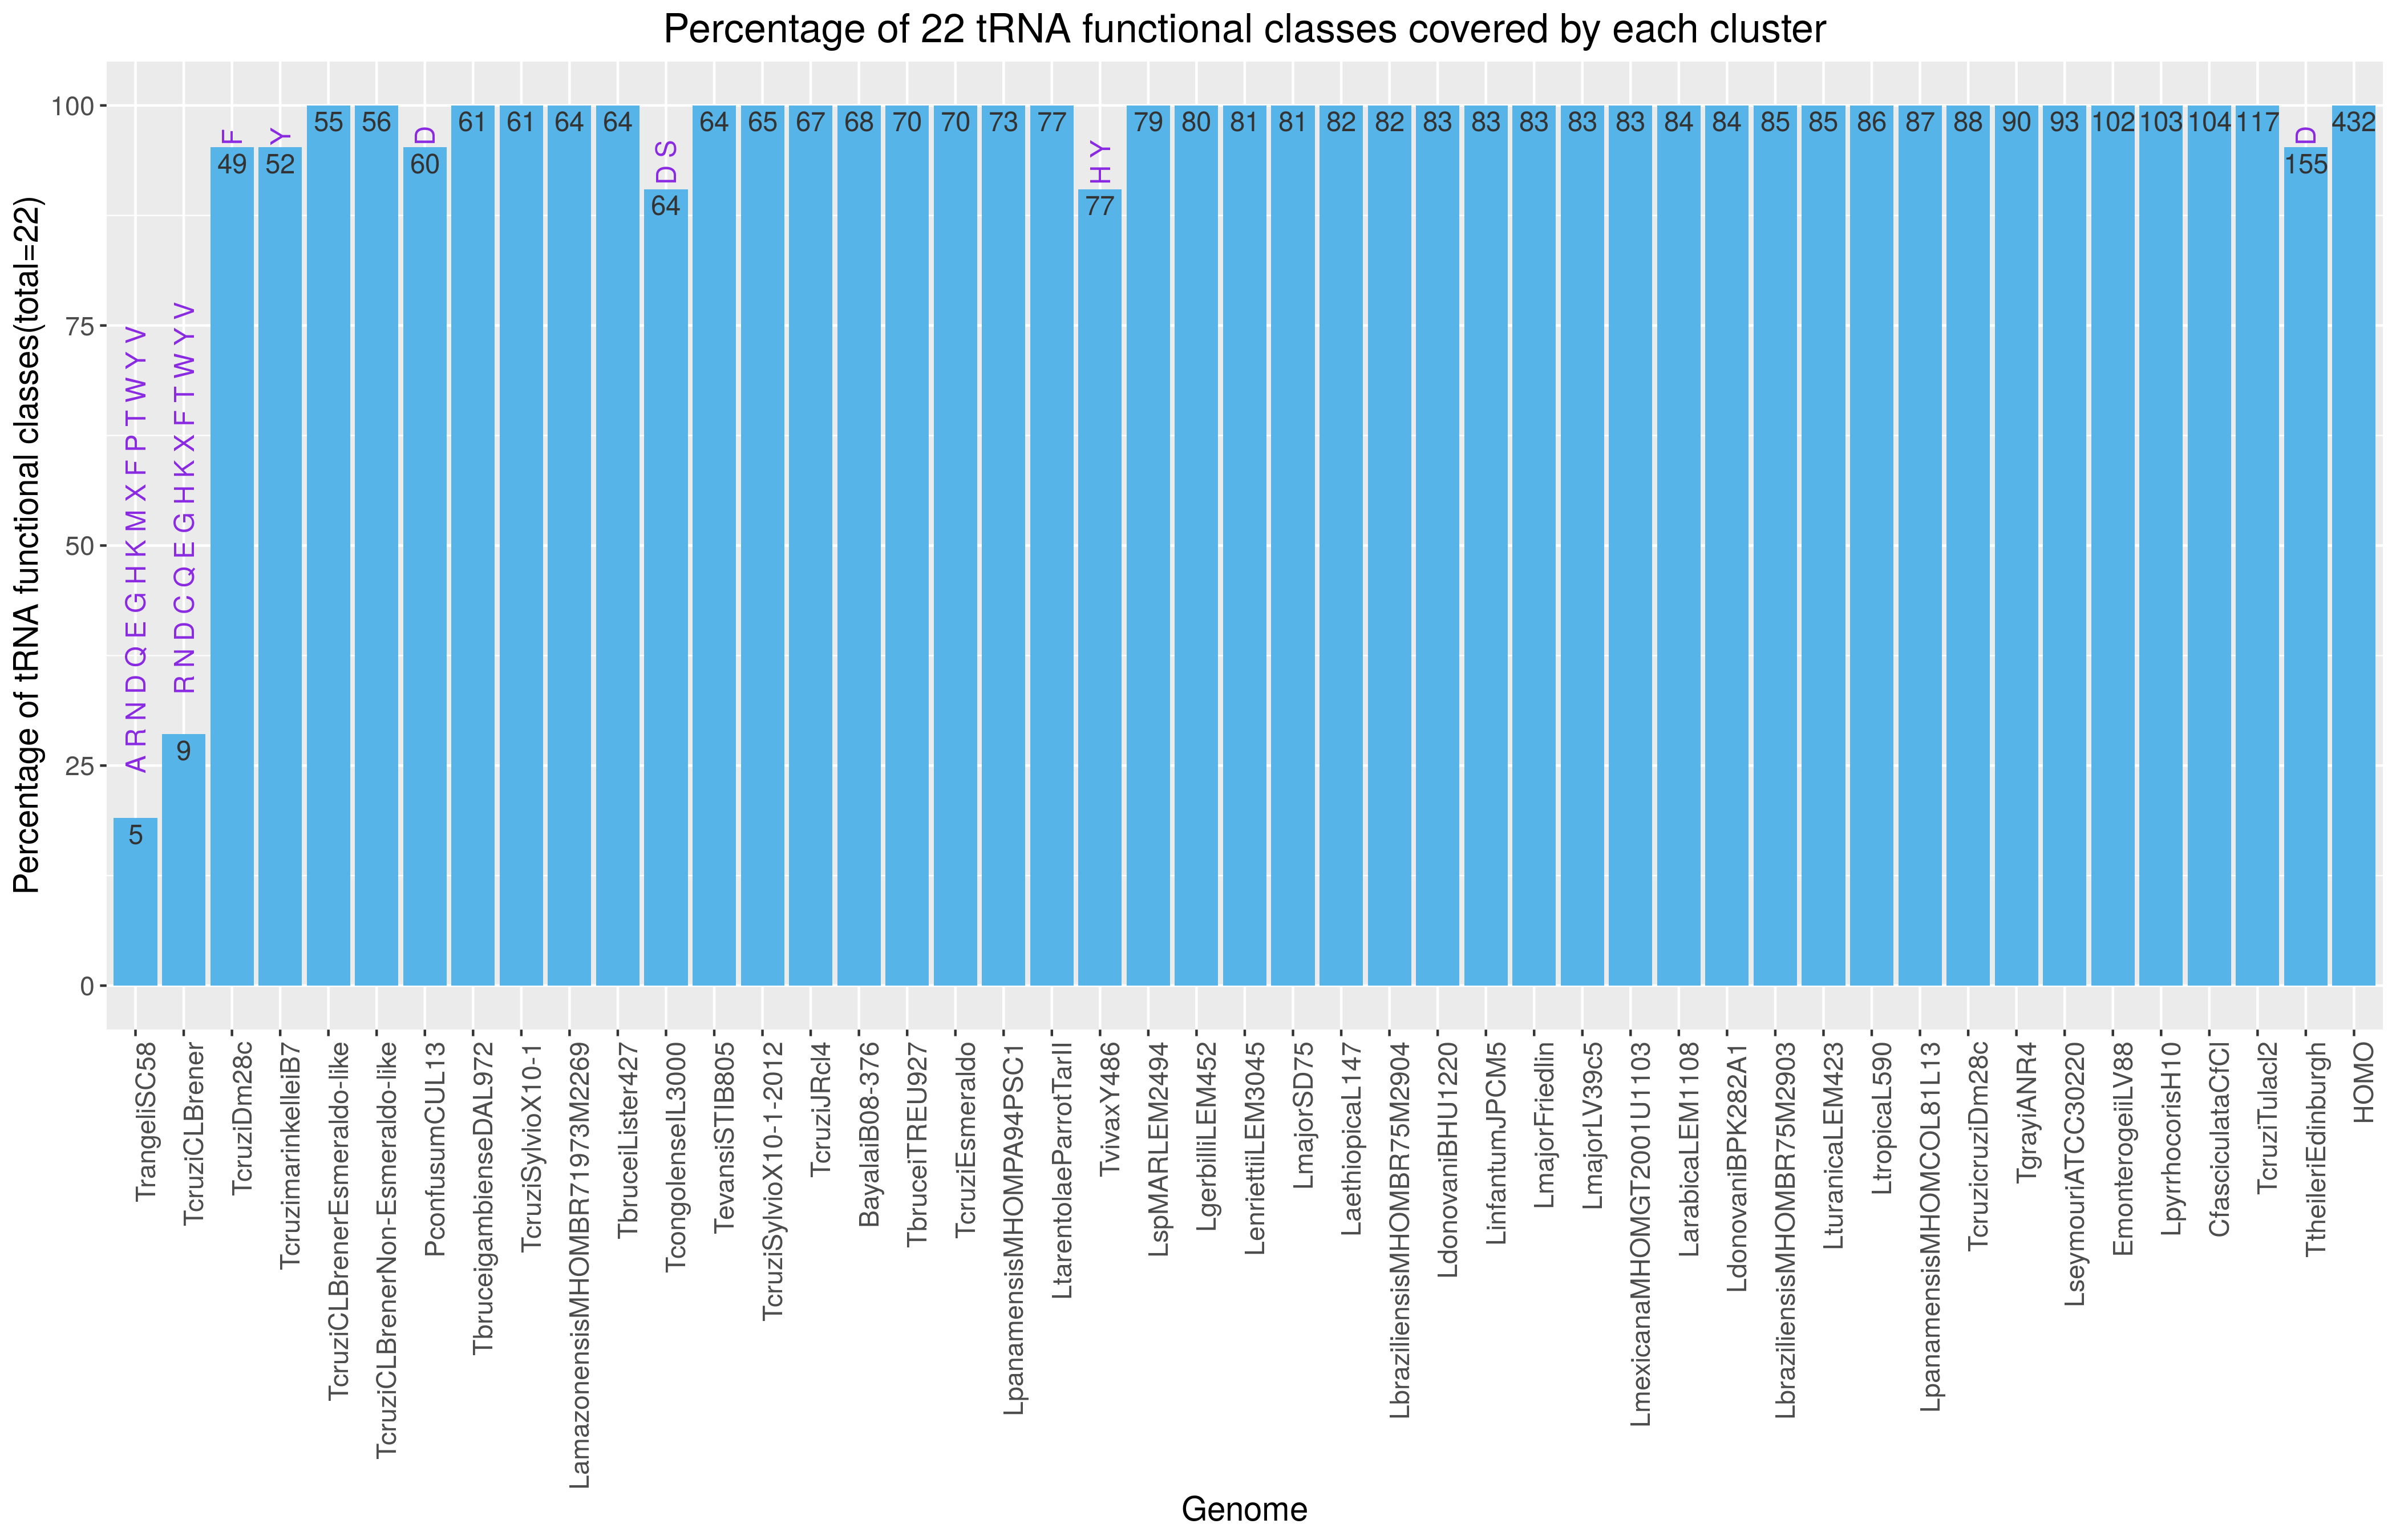
\includegraphics[width=\textwidth]{funcPerc_after.png}}}%
  \caption{Percentage of 21 predicted tRNA gene class for each genome. the missing classes are shown at the top of each bar. the numbers show the number of predicted genes for genomes. a) This figure shows the percantage of tRNA gene classes for each genome before adding 10 genes with unmatch identity between two genes finder (genes identified as Y by TSE and N by  ARA) b) This figure shows the percantage of tRNA gene classes for each genome after adding these 10 genes.}%
  \label{fig:genPerc}%
\end{figure}

\begin{table}[htbp]
  \caption{Summary of Gene Set. Last three columns are each for one gene set. Sets are defined as: a) Intersection Of two gene finders. Two genes are considered same gene if their coordinate overlaps at least one base. Displacement of overlapped genes between ARA and TSE does not pass 4bp. b) Union of two gene finders. c) Genes found by only ARA. Genes marked as \# include: pseudo|truncated genes (6 genes), genes with different predicted identity by two genefinders(23 genes), genes with unassigned identity|anticodon by any of genefinders (2 genes), and genes with letter N in their sequence(we had 4 of these genes). we also had 1 genes preicted by only TSE labeled as \# which is not shown in this table as a seperate column, however it is considered in the union set.}
  \begin{adjustbox}{center}
    %\caption{Table of Grades}
    %\centering
    \begin{tabular}{|lccc|}
      \hline
      \rowcolor{shadecolor}
      Sets            & Intersection & ARAonly & Union \\
      \hline\hline
      \#tRNA          & 3579         & 36      & 3616  \\
      \#N/\#G         & 74           & 98      & 75    \\
      Min Gene Length & 68           & 71      & 68    \\
      Max Gene Length & 89           & 206     & 206   \\
      \%intron        & 2            & 28      & 3     \\
      \%G             & 32           & 33      & 32    \\
      \%C             & 26           & 26      & 26    \\
      A               & 210          & 2       & 212   \\
      C               & 64           & 1       & 65    \\
      D               & 105          & 1       & 106   \\
      E               & 160          & 1       & 161   \\
      F               & 104          & 2       & 106   \\
      G               & 228          & 3       & 231   \\
      H               & 80           & 4       & 84    \\
      I               & 171          & 1       & 172   \\
      K               & 183          & 1       & 184   \\
      L               & 335          & 6       & 341   \\
      M               & 97           & 0       & 97    \\
      N               & 125          & 0       & 125   \\
      P               & 200          & 0       & 200   \\
      Q               & 161          & 0       & 161   \\
      R               & 348          & 2       & 350   \\
      S               & 228          & 7       & 235   \\
      T               & 218          & 4       & 222   \\
      V               & 236          & 0       & 236   \\
      W               & 52           & 1       & 53    \\
      X               & 76           & 0       & 76    \\
      Y               & 88           & 0       & 88    \\
      Z               & 76           & 0       & 76    \\
      \#              & 34           & 0       & 35    \\
      \hline
    \end{tabular}
    \label{table:genesummery}
  \end{adjustbox}
\end{table}


\begin{figure}[tb]
  \centering
  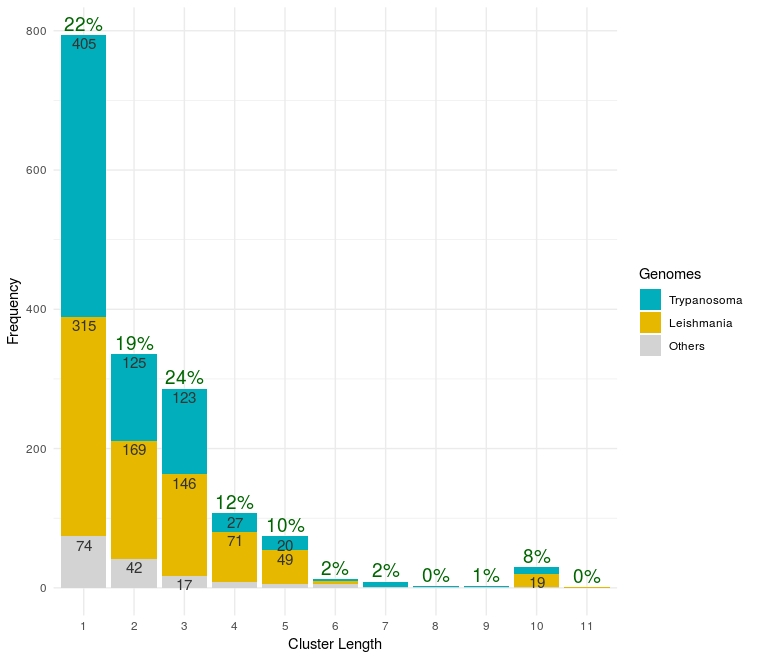
\includegraphics[width=\columnwidth]{clussize.jpeg}
  \caption[Genome Comparison]{Cluster size distribution for three categories of TryTryp genomes. Labels in green on top of each bar show the percentage of total number of genes as cluster of a specific length. Each color refers to one category of TriTryp genomes. Numbers within each color section of the bar shows the counts of clusters with a specific length.}
  \label{fig:clussize}
\end{figure}

\begin{table}[htbp]
  \caption{non-pseuso|truncated|unmatched-identity genes removed from the gene set after the applying score cutoff}
  \begin{adjustbox}{width=10cm,center}
    %\caption{Table of Grades}
    %\centering
    \begin{tabular}{|l|ccccccccccccccc|}
      \hline
      Functional Class & ? & A & C & E & G & H & I & L & M & Q & R & S & V & Y & Z \\
      Frequency        & 3 & 1 & 1 & 1 & 1 & 1 & 3 & 2 & 2 & 1 & 1 & 1 & 6 & 1 & 5 \\
      \hline
    \end{tabular}
    \label{table:removedgenes}
  \end{adjustbox}
\end{table}
%------------------------------------------------------------------------------------------------------
% Deviations between two gene finders
%------------------------------------------------------------------------------------------------------

\subsection{2.1 Criteria for filtering out genes with vague identity for creating CIFs}
For the purpose of creating CIFs, 20 genes marked with "??" were removed and genes with identity Z were excluded which left us with 3500 genes. Later, From GtRNAdb, we downloaded the last version of Homo sapiens High confidence tRNA sequences which include 433 genes with functional class distribution shown in table\ref{table:homo1} and length size distribution shown in table \ref{table:homo2}. TriTryp genes and Human genes (excluding genes with identity Z) were aligned using the alignment pipeline described in section 3 to be used as input for creating CIFs. figure \ref{fig:genPerc} shows the number of genes annotated for each genome, and the missing functional classes for each genome after the alignment.

\begin{table}[htbp]
  \caption{}
  \begin{adjustbox}{width=15cm,center}
    \begin{tabular}{|l|c c c c c c c c c c c c c c c c c c c c c c|}
      \hline
      Functional Class & A  & C  & D  & E  & F  & G  & H & I  & K  & L  & M  & N  & P  & Q  & R  & S  & T  & V  & W & X & Y  & Z \\

      Frequency        & 38 & 29 & 13 & 16 & 10 & 28 & 9 & 23 & 27 & 32 & 11 & 25 & 20 & 19 & 28 & 25 & 20 & 28 & 7 & 9 & 14 & 1 \\
      \hline
    \end{tabular}
    \label{table:homo1}
  \end{adjustbox}
\end{table}


\begin{table}[htbp]
  \caption{}
  \begin{adjustbox}{width=7cm,center}
    \begin{tabular}{|l|c c c c c c|}
      \hline
      Gene Length & 70 & 71 & 72  & 73  & 74 & 75 \\
      Frequency   & 1  & 20 & 151 & 118 & 60 & 1  \\
      \hline
    \end{tabular}
    \label{table:homo2}
  \end{adjustbox}
\end{table}


%------------------------------------------------------------------------------------------------------
% Deviations between two gene finders
%------------------------------------------------------------------------------------------------------
\section{TryTryp Classification}

Using phylogenetic trees of Trypanosoma from these works \cite{Souza:2018dg,Hughes:2003,Pothirat:2014,Kelly:2017}, we grouped TryTryp genomes as table \ref{table:Genomeclusters1}.\\
\begin{table}[hbt]
  \caption{Classification of TryTryp genomes. genomes not mentioned here are clustered as one genome.}
  \begin{adjustbox}{width=\columnwidth,center}
    \begin{tabular}{|c|c|c|c|c|c|c|c|}
      \toprule LenriettiComplex                           & AfricanTrypanosome (T1)                            & AmericanTrypanosome (T2)                           & Leishmania1                                        & Leishmania2                                        & Leishmania3                                        & Leishmania4                                        & Leishmania5 (Lvianna)                              \\\midrule
      \parbox{.45\textwidth} {\begin{enumerate}
          \item LspMARLEM2494
          \item LenriettiiLEM3045
        \end{enumerate}} & \parbox{.45\textwidth}{\begin{enumerate}
          \item TbruceigambienseDAL972
          \item TbruceiLister427
          \item TbruceiTREU927
          \item TevansiSTIB805
          \item TcongolenseIL3000
          \item TvivaxY486
        \end{enumerate}} & \parbox{.45\textwidth}{\begin{enumerate}
          \item TgrayiANR4
                %\item TrangeliSC58
                %\item TcruziCLBrener
          \item TcruziCLBrenerEsmeraldo-like
          \item TcruziCLBrenerNon-Esmeraldo-like
          \item TcruzicruziDm28c
          \item TcruziDm28c
          \item TcruziEsmeraldo
          \item TcruziJRcl4
          \item TcruzimarinkelleiB7
          \item TcruziSylvioX10-1
          \item TcruziSylvioX10-1-2012
          \item TcruziTulacl2
                %\item TtheileriEdinburgh
        \end{enumerate}} & \parbox{.45\textwidth}{\begin{enumerate}
          \item CfasciculataCfCl
          \item LseymouriATCC30220
          \item LpyrrhocorisH10
        \end{enumerate}} & \parbox{.45\textwidth}{\begin{enumerate}
          \item Lamazonensis\\
                MHOMBR71973M2269
          \item Lmexicana\\MHOMGT2001U1103
        \end{enumerate}} & \parbox{.45\textwidth}{\begin{enumerate}  % trusted
          \item LmajorFriedlin
          \item LmajorLV39c5
          \item LmajorSD75
          \item LturanicaLEM423
          \item LarabicaLEM1108
          \item LtropicaL590
          \item LaethiopicaL147
          \item LgerbilliLEM452
        \end{enumerate}} & \parbox{.45\textwidth}{\begin{enumerate} % trusted
          \item LdonovaniBHU1220
          \item LdonovaniBPK282A1
          \item LinfantumJPCM5
        \end{enumerate}} & \parbox{.45\textwidth}{\begin{enumerate}  % trusted
          \item Lbraziliensis\\MHOMBR75M2904
          \item Lbraziliensis\\MHOMBR75M2903
          \item Lpanamensis\\MHOMPA94PSC1
          \item Lpanamensis\\MHOMCOL81L13
        \end{enumerate}} \\
      \bottomrule
    \end{tabular}
    \label{table:Genomeclusters1}
  \end{adjustbox}
\end{table}

\newpage
%\subsubsection{2.1.1 summery of final gene set}
%...\\
%...
%------------------------------------------------------------------------------------------------------
% Deviations between two gene finders
%------------------------------------------------------------------------------------------------------

\section{3. Alignment pipeline}
...\\
...
%------------------------------------------------------------------------------------------------------
% Deviations between two gene finders
%------------------------------------------------------------------------------------------------------

\section{4. CIF Results}

...\\
...
%------------------------------------------------------------------------------------------------------
% Deviations between two gene finders
%------------------------------------------------------------------------------------------------------


%----------------------------------------------------------------------------------------
% BIBLIOGRAPHYyour own dat
%----------------------------------------------------------------------------------------
\newpage
\
\renewcommand{\refname}{\spacedlowsmallcaps{References}} % For modifying the bibliography heading

\bibliographystyle{unsrt}

\bibliography{sample.bib} % The file containing the bibliography

%----------------------------------------------------------------------------------------

\end{document}
